\documentclass{beamer}

\mode<presentation> { 
% The Beamer class comes with a number of default slide themes
% which change the colors and layouts of slides. Below this is a list
% of all the themes, uncomment each in turn to see what they look like.

%\usetheme{default}
\usetheme{AnnArbor}
%\usetheme{Antibes}
%\usetheme{Bergen}
%\usetheme{Berkeley}
%\usetheme{Berlin}
%\usetheme{Boadilla}
%\usetheme{CambridgeUS}
%\usetheme{Copenhagen}
%\usetheme{Darmstadt}
%\usetheme{Dresden}
%\usetheme{Frankfurt}
%\usetheme{Goettingen}
%\usetheme{Hannover}
%\usetheme{Ilmenau}
%\usetheme{JuanLesPins}
%\usetheme{Luebeck}
%\usetheme{Madrid}
%\usetheme{Malmoe}
%\usetheme{Marburg}
%\usetheme{Montpellier}
%\usetheme{PaloAlto}
%\usetheme{Pittsburgh}
%\usetheme{Rochester}
%\usetheme{Singapore}
%\usetheme{Szeged}
%\usetheme{Warsaw}

% As well as themes, the Beamer class has a number of color themes
% for any slide theme. Uncomment each of these in turn to see how it
% changes the colors of your current slide theme.

%\usecolortheme{albatross}
%\usecolortheme{beaver}
%\usecolortheme{beetle}
\usecolortheme{crane}
%\usecolortheme{dolphin}
%\usecolortheme{dove}
%\usecolortheme{fly}
%\usecolortheme{lily}
%\usecolortheme{orchid}
%\usecolortheme{rose}
%\usecolortheme{seagull}
%\usecolortheme{seahorse}
%\usecolortheme{whale}
%\usecolortheme{wolverine}

%\setbeamertemplate{footline} % To remove the footer line in all slides uncomment this line
%\setbeamertemplate{footline}[page number] % To replace the footer line in all slides with a simple slide count uncomment this line

%\setbeamertemplate{navigation symbols}{} % To remove the navigation symbols from the bottom of all slides uncomment this line
}

\usepackage{graphicx} % Allows including images
\usepackage{booktabs} % Allows the use of \toprule, \midrule and \bottomrule in tables
\usepackage{epstopdf,epsfig}
\usepackage{amsthm}
\usepackage{amsmath}
\usepackage{mathtools}
\usepackage{tikz}
\usepackage{cancel}
\usepackage{comment}
\usepackage[normalem]{ulem}
\usetikzlibrary{arrows, automata, shapes,positioning}
\usepackage{listings}
\lstset{language=Haskell}

\tikzset{onslide/.code args={<#1>#2}{%
  \only<#1>{\pgfkeysalso{#2}} % \pgfkeysalso doesn't change the path
}}



\graphicspath{{./}{../img}}

%----------------------------------------------------------------------------------------
%	TITLE PAGE
%----------------------------------------------------------------------------------------


\title[MBT]{Test and verification techniques in conformance checking} % The
% short title appears at the bottom of every slide, the full title is only on the title page

\author{Kevin Jahns} % Your name
\institute[] % Your institution as it will appear on the bottom of every
% slide, may be shorthand to save space
{
RWTH Aachen University \\ % Your institution for the title page
\medskip
\textit{kevin.jahns@rwth-aachen.de} % Your email address
}
\date{\today} % Date, can be changed to a custom date

\begin{document}
\begin{frame}
\titlepage % Print the title page as the first slide
\end{frame}

\begin{frame}
\frametitle{Overview} % Table of contents slide, comment this block out to remove it
\tableofcontents % Throughout your presentation, if you choose to use \section{} and \subsection{} commands, these will automatically be printed on this slide as an overview of your presentation
\end{frame}

%----------------------------------------------------------------------------------------
%	PRESENTATION SLIDES
%----------------------------------------------------------------------------------------

\section{Why testing}

%------------------------------------------------
\section{Conformance} % Sections can be created in order to organize your
% presentation into discrete blocks, all sections and subsections are automatically printed in the table of contents as an overview of the talk ------------------------------------------------

\begin{frame}
\frametitle{What is \textit{conformance}?}
    \begin{columns}[c] % the "c" option specifies center vertical alignment
    \column{.5\textwidth} % column designated by a command
    	\begin{block}{Conformance is ..}
        \begin{enumerate}[(1)]
          \item<2-> when it does not throw errors?
          \item<3-> whet it works for the developer (everything else is a user
          error)?
          \item<4-> when it works for the user?
          \item<5-> when it does not explode ;) 
          \item<6-> whet it conforms to some sort of specification?
          \item[$\xrightarrow{\ }$]<7-> Conformance is hard to express
        \end{enumerate}
        \end{block}
    \column{.5\textwidth}
            \includegraphics[width=\textwidth]{../img/perfect_remote_control}
    \end{columns}
\end{frame}

\begin{frame}
\frametitle{How to check conformance}

\Large{Expressing conformance $\xrightarrow{\ }$ checking conformance}

\end{frame}

\begin{frame}
\frametitle{Test vs. verification}
\begin{block}{Test}
You \textit{may} find an error after the execution of a test.
\end{block}
\begin{block}{Verification}
The evaluation of whether or not something complies with a
specified conformance property
\end{block}
\end{frame}

\begin{frame}
\frametitle{Testing a robot}

    \begin{columns}[c] % the "c" option specifies center vertical alignment
    \column{.5\textwidth} % column designated by a command
    \begin{block}{Test \color{red}``Don't kill me''}
    \begin{itemize}
      \item If the robot kills you, you can be sure that the property is not fulfilled.
    \end{itemize}
    \end{block}
    \column{.5\textwidth}
    \includegraphics[width=\textwidth]{../img/robot}
    \end{columns}
\end{frame}

\begin{frame}
\frametitle{Verifying a robot}

    \begin{columns}[c] % the "c" option specifies center vertical alignment
    \column{.5\textwidth} % column designated by a command
    \begin{block}{Test \color{red}``Don't kill me''}
    \begin{itemize}
      \item After verifying that a robot won't kill you, he will not kill you
      ;)
    \end{itemize}
    \end{block}
    \column{.5\textwidth}
    \includegraphics[width=\textwidth]{../img/robot}
    \end{columns}
\end{frame}

\begin{frame}
\frametitle{Monkey testing}
    \begin{columns}[c] % the "c" option specifies center vertical alignment
    \column{.5\textwidth} % column designated by a command
\begin{block}{Infinite monkey theorem}
The \textbf{infinite monkey theorem} states that a monkey hitting keys at random
on a typewriter keyboard for an infinite amount of time will almost surely type a
given text, such as the complete works of William Shakespeare.\cite{monkey}
\end{block}
    \column{.5\textwidth}
    \includegraphics[width=\textwidth]{../img/monkey_approach} 
    \end{columns}
\end{frame}

\begin{frame}[fragile]
\frametitle{Model checking}
    \begin{columns}[c] % the "c" option specifies center vertical alignment
    \column{.5\textwidth} % column designated by a command
    \lstset{basicstyle=\footnotesize,showspaces=false,numbers=right, numbers=left, numbersep=-7pt,
    numberstyle=\small, showstringspaces=false}
    \begin{lstlisting}
  main = do
    putStrLn $ 
         "What is the the"
      ++ "answer to life"
      ++ "the universe"
      ++ "and everything?"
    answer <- getLine
    case answer of 
      "42" -> 
        putStrLn 
           "You're right"
      _	 -> 
        putStrLn 
           "Nope"
    main 
    \end{lstlisting}
    \column{.5\textwidth}
    \begin{figure}
    \label{simpleTS}
    \capition{Simple transition system}
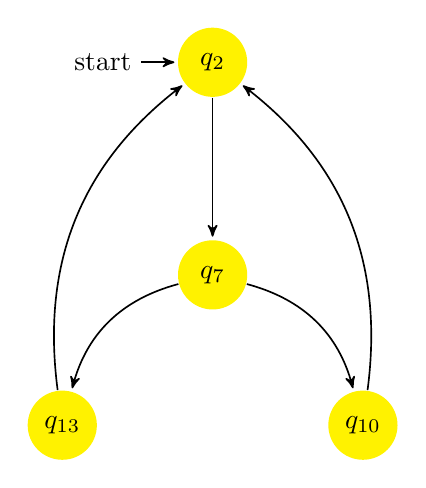
\begin{tikzpicture}[->,>=stealth',shorten >=1pt,auto,node distance=2.7cm,
                    semithick, main node/.style={font=\small}]
  \tikzstyle{every state}=[fill=yellow,draw=none,text=black]

  \node[initial,state] (AA)                    {$q_2$};
  \node[state]         (A)[below of=AA]       {$q_7$};
  \node[state]         (B) [below right of=A] {$q_{10}$};
  \node[state]         (D) [below left of=A] {$q_{13}$};

  \path[every node/.style={font=\tiny}] 
        (AA)edge              node {} (A)
        (A) edge [bend left]  node {} (B)
        (A) edge [bend right] node {} (D)
        (D) edge [bend left]  node {} (AA)
        (B) edge [bend right] node {} (AA);

\end{tikzpicture}    
    \end{figure}
\end{columns}
\end{frame}

\begin{frame}[fragile]
\frametitle{Complexety of model checking}
\begin{center}
{\small
\begin{tabular}{|p{3.3cm}|p{3.3cm}|p{3.3cm}|}
    \hline
    Real world TS &  & \textit{thousands} of states\\ \hline
    \onslide<2->{Each State depends on the variables of the Programm & Real
    world programs have thousands of variables & dimension of new TS $\approx
    1000^{1000}$} \\
    \hline
    \onslide<3->{Time complexety of model checking algorithm is NP-hard &
    $O(2^{TS})$ computation steps & $\approx 2^{1000^{1000}} \approx
    10^{10^{3000}} cumputation steps$}\\
    \hline
    \onslide<4->{Number of atoms in the entire observable universe & &
    $10^{80}$}\\
    \hline
    
\end{tabular}}
\end{center}
\end{frame}

\begin{frame}
\frametitle{References}
%\bibliographystyle{unsrt}
%\bibliographystyle{abbrvnat}
%\bibliographystyle{apacite}
\bibliographystyle{plain}
\bibliography{../sample}
\end{frame}

%------------------------------------------------

\begin{frame}
\Huge{\centerline{The End}}
\end{frame}
%----------------------------------------------------------------------------------------

\end{document} 
